\documentclass{beamer}
\usepackage{etex}
\usetheme{default}
\usecolortheme{seagull}
\usefonttheme{structurebold}
\usenavigationsymbolstemplate{}

\definecolor{paprika}{rgb}{0.6,0,0.2}
\definecolor{pineglade}{rgb}{0.95,0.95,0.75}

\setbeamercolor{structure}{fg=paprika}
\setbeamercolor{block title}{fg=paprika,bg=pineglade}
\setbeamercolor{alerted text}{fg=paprika}
\setbeamercolor{block body}{bg=pineglade}
\setbeamertemplate{title page}
{%
   \begin{center}
      \begin{minipage}{0.9\textwidth}
         \begin{block}{}
            \begin{center}
              \Large{\alert{\inserttitle}}\\
              \large{\alert{\insertsubtitle}}\\
               \vspace{0.5cm}
               \large{\insertauthor}\\
               \large{\texttt{melissa.mendonca@ufsc.br}}
            \end{center}
         \end{block}
      \end{minipage}
   \end{center}
}

\usepackage[portuguese]{babel}
\usepackage[utf8]{inputenc} % To use characters such as é without typing é
\usepackage{tikz}
\usetikzlibrary{positioning}
\usetikzlibrary{arrows, decorations.markings}
% for double arrows a la chef
\tikzstyle{vecArrow} = [thick, paprika, decoration={markings,mark=at position
   1 with {\arrow[semithick,paprika]{open triangle 60}}},
   double distance=1.4pt, shorten >= 5.5pt,
   preaction = {decorate},
   postaction = {draw,line width=1.4pt, pineglade,shorten >= 4.5pt}]
% Define box and box title style
\tikzstyle{mybox} = [draw, very thick, rectangle,rounded corners, inner sep=10pt, inner ysep=20pt]
\usepackage{ctable} % provides \toprule,\bottomrule,\midrule for tables

\newcommand{\kw}[1]{\alert{\texttt{#1}}}
\newcommand{\code}[1]{{\texttt{#1}}}
\newcommand{\acode}[1]{\alert{\texttt{#1}}}
\newcommand{\codigo}[1]{\begin{center}\rm{\code{
  \begin{tabular}{r l}
  #1
  \end{tabular}
  }}\end{center}}
\newcommand{\ac}{\alert{\texttt{>>}}}
\newcommand{\file}[3]{\texttt{
   \begin{center}
      \begin{tikzpicture}
         \node[mybox] (box) {
            \begin{minipage}{#1}
               #3
            \end{minipage}
         };
         \node[draw, fill=white, text=black, right=10pt, rounded corners] at (box.north west) {
            \textbf{#2}
         };
      \end{tikzpicture}
   \end{center}}
}

\title{MATLAB Avançado}
\subtitle{Aula 4}
\author[M. Weber Mendonça]{Melissa Weber Mendonça}
\institute[UFSC]{\inst{1} Universidade Federal de Santa Catarina} 
\date{2014.1}

\logo{
\includegraphics[height=1.5cm]{img/brasao_UFSC.png}}

\begin{document}
%%%
% Slide 1
\begin{frame}
% Title
  \titlepage
\end{frame}
%%%%%%%%%%%%%%%%%%%%%%%%%%%%%%%%%%%%%%%%%%%%%%%%%%%%%%%%%%%%%%%%%%%%%%%%%%%%%%%%%%%%%%%%%
\begin{frame}
  \frametitle{Fitting}
  Queremos descobrir uma função (linear, polinomial ou não-linear) que aproxime um conjunto de dados:
  \begin{center}
    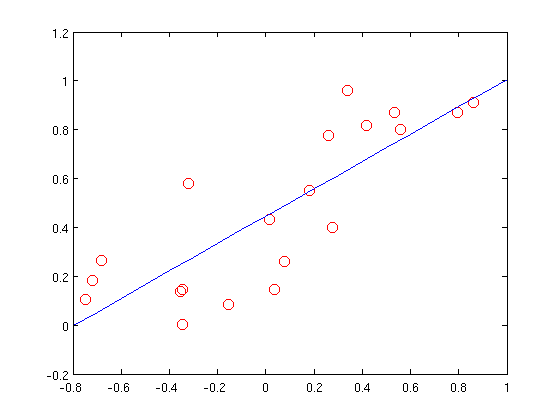
\includegraphics[width=6cm]{img/fit.png}
  \end{center}
\end{frame}
%%%%%%%%%%%%%%%%%%%%%%%%%%%%%%%%%%%%%%%%%%%%%%%%%%%%%%%%%%%%%%%%%%%%%%%%%%%%%%%%%%%%%%%%%
\begin{frame}
   \frametitle{Regressão}

   Podemos calcular automaticamente um modelo de regressão (usando quadrados mínimos) através da janela de um gráfico.

   Exemplo:
   \codigo{\ac & \acode{load} census\\
      \ac & \acode{plot}(cdate, pop, 'ro')}

   Na janela do gráfico, podemos selecionar
   \begin{center}
      Tools $\rightarrow$ Basic Fitting
   \end{center}
\end{frame}
%%%%%%%%%%%%%%%%%%%%%%%%%%%%%%%%%%%%%%%%%%%%%%%%%%%%%%%%%%%%%%%%%%%%%%%%%%%%%%%%%%%%%%%%%
\begin{frame}
   \frametitle{Norma dos resíduos}
   Podemos calcular a norma dos resíduos para um \emph{fit} realizado através do comando
   \codigo{\ac & \acode{sqrt}(\acode{sum}(resids.\^{}2))}

   Podemos também extrapolar dados usando a interface gráfica do MATLAB, novamente em 
   \begin{center}
      Tools $\rightarrow$ Basic Fitting
   \end{center}
   Finalmente, podemos usar o comando 
   \begin{center}
      File $\rightarrow$ Generate Code
   \end{center}
   para criarmos uma função que reproduz o gráfico obtido.
\end{frame}
%%%%%%%%%%%%%%%%%%%%%%%%%%%%%%%%%%%%%%%%%%%%%%%%%%%%%%%%%%%%%%%%%%%%%%%%%%%%%%%%%%%%%%%%%
\begin{frame}
   \frametitle{Interpolação polinomial: \code{polyfit}}
   O comando
   \codigo{\ac & p = \acode{polyfit}(x,y,n)}
   encontra os coeficientes do polinômio $p(x)$ de grau $n$ que aproxima os dados $y(i)=p(x(i))$, em um sentido de mínimos quadrados. O vetor \code{p} resultante contém os coeficientes do polinômio em ordem descendente de potências.
   O comando
   \codigo{\ac &[p,S] = \acode{polyfit}(x,y,n)}
   retorna os coeficientes do polinômio em \code{p} e uma estrutura \code{S} que pode ser usada com o comando \acode{polyval}. 

   A estrutura \code{S} contém os campos \code{R}, \code{df} e \code{normr}.

   Se os dados \code{y} são aleatórios, uma estimativa da covariância de \code{p} é
   \codigo{\ac &  (\acode{inv}(R)*\acode{inv}(R)')*\acode{normr}\^{}2/df}
\end{frame}
%%%%%%%%%%%%%%%%%%%%%%%%%%%%%%%%%%%%%%%%%%%%%%%%%%%%%%%%%%%%%%%%%%%%%%%%%%%%%%%%%%%%%%%%%
\begin{frame}
   \frametitle{Avaliação de polinômios: \code{polyval}}
   O comando
   \codigo{\ac & y = \acode{polyval}(p,x)}
   retorna o valor de um polinômio de grau \code{n} (armazenado no vetor \code{p}) em \code{x}.
   O comando 
   \codigo{\ac & [y,delta] = \acode{polyval}(p,x,S)}
   usa a estrutura \code{S} gerada pelo comando \acode{polyfit} para gerar \code{delta}, que é uma estimativa do desvio padrão do erro obtido ao se tentar calcular \code{p(x)}. 
\end{frame}
%%%%%%%%%%%%%%%%%%%%%%%%%%%%%%%%%%%%%%%%%%%%%%%%%%%%%%%%%%%%%%%%%%%%%%%%%%%%%%%%%%%%%%%%%
\begin{frame}
  \frametitle{Regressão por Quadrados Mínimos}
  Por exemplo, se quisermos fazer uma regressão linear em um conjunto de pontos $(x,y)$, usamos o comando
  \codigo{\ac & p = \acode{polyfit}(x,y,1)}
  O resultado é um vetor \code{p} que contém os coeficientes da reta
  $$y = p_1x+p_2$$
  \vfill
  Exemplo:
  \codigo{\ac & x = 1:1:20;\\
    \ac & y = x + 10*\acode{rand}(1,20);\\
    \ac & p = \acode{polyfit}(x,y,1);\\
    \ac & \acode{plot}(x,y,'ro')\\
    \ac & \acode{hold on}\\
    \ac & t = 0:0.1:20;\\
    \ac & \acode{plot}(t,\acode{polyval}(p,t))}
\end{frame}
%%%%%%%%%%%%%%%%%%%%%%%%%%%%%%%%%%%%%%%%%%%%%%%%%%%%%%%%%%%%%%%%%%%%%%%%%%%%%%%%%%%%%%%%%
\begin{frame}
  \frametitle{Exemplo (com resíduos)}
  \codigo{\ac & x = 1:1:20;\\
    \ac & y = x + 10*\acode{rand}(1,20);\\
    \ac & p = \acode{polyfit}(x,y,1);\\
    \ac & fitted = \acode{polyval}(p,x);\\
    \ac & res = y-fitted;\\
    \ac & \acode{subplot}(2,1,1), \acode{plot}(x,y,'ro','markersize',8)\\
    \ac & \acode{hold on}\\
    \ac & t = 0:0.1:20;\\
    \ac & \acode{subplot}(2,1,1), \acode{plot}(t,\acode{polyval}(p,t))\\
    \ac & \acode{subplot}(2,1,2), \acode{bar}(x,res)}  
\end{frame}
%%%%%%%%%%%%%%%%%%%%%%%%%%%%%%%%%%%%%%%%%%%%%%%%%%%%%%%%%%%%%%%%%%%%%%%%%%%%%%%%%%%%%%%%%
\begin{frame}
   \frametitle{Scatter Plot}
   O comando
   \codigo{\ac & \acode{scatter}(X,Y)}
   faz um gráfico dos pontos com coordenadas \code{X} e \code{Y}, usando círculos como marcadores.
   
   Se usarmos
   \codigo{\ac & \acode{scatter}(X,Y,S,C)}
   podemos especificar a área de cada marcador em \code{S}. 

   Outras opções:
   \begin{itemize}
      \item \acode{scatter}\code{(...,marcador)} usa o marcador escolhido (p. ex. \code{'+'} ou \code{'*'})
      \item \acode{scatter}\code{(...,'filled')} preenche os marcadores.
   \end{itemize}
\end{frame}
%%%%%%%%%%%%%%%%%%%%%%%%%%%%%%%%%%%%%%%%%%%%%%%%%%%%%%%%%%%%%%%%%%%%%%%%%%%%%%%%%%%%%%%%%
\begin{frame}
   \frametitle{\code{scatterhist}}
   O comando
   \codigo{\ac & \acode{scatterhist}(x,y)}
   cria um \emph{scatter plot} dos dados nos vetores \code{x} e \code{y} e também um histograma em cada eixo do gráfico. 
   \vfill
   Exemplo: 
   
   \codigo{\ac & x = \acode{randn}(1000,1);\\
      \ac & y = \acode{exp}(.5*\acode{randn}(1000,1));\\
      \ac & \acode{scatterhist}(x,y)}
\end{frame}
%%%%%%%%%%%%%%%%%%%%%%%%%%%%%%%%%%%%%%%%%%%%%%%%%%%%%%%%%%%%%%%%%%%%%%%%%%%%%%%%%%%%%%%%%
\begin{frame}
  \frametitle{\code{lsline}}

  O comando
  \codigo{\ac & \acode{lsline}}
  acrescenta uma reta calculada através de regressão linear (mínimos quadrados) \alert{para cada plot/scatter plot na figura atual}. 
\vfill
  Atenção: dados conectados com alguns tipos de reta (\code{'-'}, \code{'--'} ou \code{'.-'}) são \alert{ignorados} por \acode{lsline}.
\end{frame}
%%%%%%%%%%%%%%%%%%%%%%%%%%%%%%%%%%%%%%%%%%%%%%%%%%%%%%%%%%%%%%%%%%%%%%%%%%%%%%%%%%%%%%%%%
\begin{frame}
  \frametitle{Exemplo}
  \codigo{\ac & x = 1:10;\\
     \ac & y1 = x + \acode{randn}(1,10);\\
     \ac & \acode{scatter}(x,y1,25,'b','*')\\
     \ac & \acode{hold on}\\
     \ac & y2 = 2*x + \acode{randn}(1,10);\\
     \ac & \acode{plot}(x,y2,'mo')\\
     \ac & y3 = 3*x + \acode{randn}(1,10);\\
     \ac & \acode{plot}(x,y3,'rx:')\\
     \ac & y4 = 4*x + \acode{randn}(1,10);\\
     \ac & \acode{plot}(x,y4,'g+--')\\
     \ac & \acode{lsline}}
\end{frame}
%%%%%%%%%%%%%%%%%%%%%%%%%%%%%%%%%%%%%%%%%%%%%%%%%%%%%%%%%%%%%%%%%%%%%%%%%%%%%%%%%%%%%%%%%
\begin{frame}
   \frametitle{\code{refcurve}}

   Se o vetor \code{p} contém os coeficientes de um polinômio em ordem descendente de potências, o comando
   \codigo{\ac & \acode{refcurve}(p)}
   adiciona uma curva de referência polinomial com coeficientes \code{p} ao gráfico atual.

   Se \code{p} é um vetor com $n+1$ elementos, a curva é dada por
   \begin{equation*}
      y = p(1)x^n + p(2)x^{n-1} + \ldots + p(n)x + p(n+1)
   \end{equation*}
\end{frame}
%%%%%%%%%%%%%%%%%%%%%%%%%%%%%%%%%%%%%%%%%%%%%%%%%%%%%%%%%%%%%%%%%%%%%%%%%%%%%%%%%%%%%%%%%
\begin{frame}
   \frametitle{\code{gline}}

   O comando
   \codigo{\ac & \acode{gline}}
   permite ao usuário adicionar manualmente um segmento de reta à última figura desenhada.
   \vfill
   A reta pode ser editada manualmente na ferramenta de edição de gráficos do MATLAB.
\end{frame}
%%%%%%%%%%%%%%%%%%%%%%%%%%%%%%%%%%%%%%%%%%%%%%%%%%%%%%%%%%%%%%%%%%%%%%%%%%%%%%%%%%%%%%%%%
\begin{frame}
   \frametitle{Ajuste polinomial}
   O comando
   \codigo{\ac & \acode{polytool}(x,y)}
   ajusta uma reta aos vetores \code{x} e \code{y} e mostra um gráfico interativo do resultado.
   \codigo{\ac & \acode{polytool}(x,y,n)}
   ajusta um polinômio de grau \code{n} aos dados.
   \vfill
   \alert{Só disponível na Statistics Toolbox!}
\end{frame}
%%%%%%%%%%%%%%%%%%%%%%%%%%%%%%%%%%%%%%%%%%%%%%%%%%%%%%%%%%%%%%%%%%%%%%%%%%%%%%%%%%%%%%%%%
\begin{frame}
   \frametitle{Curve Fitting Toolbox}
   Para fazermos o ajuste de curvas de maneira interativa, podemos usar o comando 
   \codigo{\ac & \acode{cftool}}

   \vfill
   \alert{Só disponível com a Curve Fitting Toolbox}
\end{frame}
%%%%%%%%%%%%%%%%%%%%%%%%%%%%%%%%%%%%%%%%%%%%%%%%%%%%%%%%%%%%%%%%%%%%%%%%%%%%%%%%%%%%%%%%%
\begin{frame}
   \frametitle{}
   \begin{center}
      \alert{Resolução de equações lineares e não-lineares em MATLAB}
   \end{center}
\end{frame}
%%%%%%%%%%%%%%%%%%%%%%%%%%%%%%%%%%%%%%%%%%%%%%%%%%%%%%%%%%%%%%%%%%%%%%%%%%%%%%%%%%%%%%%%%
\begin{frame}
   \frametitle{Comandos básicos de álgebra linear: \code{det}}
 
   Para calcularmos o determinante de uma matriz quadrada \code{A}, usamos o comando
   \codigo{\ac & \acode{det}(A)}
   \vfill
   Exemplo:
   \codigo{\ac & A = [1 2 0; 3 1 4; 5 2 1]\\
   \ac & \acode{det}(A)\\
   \ac & B = [1 2 3;4 5 6;7 8 9]\\
   \ac & \acode{det}(B)}
\end{frame}
%%%%%%%%%%%%%%%%%%%%%%%%%%%%%%%%%%%%%%%%%%%%%%%%%%%%%%%%%%%%%%%%%%%%%%%%%%%%%%%%%%%%%%%%%
\begin{frame}
   \frametitle{Comandos básicos de álgebra linear: \code{eig}}
   Para calcularmos os autovalores de \code{A}, usamos
   \codigo{\ac & \acode{eig}(A)}
   Para calcularmos também os autovetores, usamos
   \codigo{\ac & [V,D] = \acode{eig}(A)}
   onde \code{V} tem os autovetores de \code{A} nas colunas, e \code{D} é uma diagonal com os autovalores de \code{A}.

   Exemplos:
   \codigo{\ac & \acode{eig}(\acode{eye}(n,n))\\
   \ac & [V,D] = \acode{eig}(\acode{eye}(n,n))\\
   \ac & A = [1 2 3;4 5 6;7 8 9];\\
   \ac & [V,D] = \acode{eig}(A)}
\end{frame}
%%%%%%%%%%%%%%%%%%%%%%%%%%%%%%%%%%%%%%%%%%%%%%%%%%%%%%%%%%%%%%%%%%%%%%%%%%%%%%%%%%%%%%%%%
\begin{frame}
   \frametitle{Comandos básicos de álgebra linear: \code{inv}}

   Para calcularmos a inversa de uma matriz \emph{quadrada e inversível} \code{A}, usamos o comando
   \codigo{\ac & \acode{inv}(A)}
   \vfill
   Exemplos:
   \codigo{\ac & M = [1 4 3;2 1 0;0 0 1];\\
     \ac & \acode{inv}(M)\\
     \ac & \acode{inv}(M)*M\\
     \ac & A = [1 2 3;4 5 6;7 8 9];\\
     \ac & \acode{inv}(A)\\
     \ac & \acode{inv}(A)*A}
\end{frame}
%%%%%%%%%%%%%%%%%%%%%%%%%%%%%%%%%%%%%%%%%%%%%%%%%%%%%%%%%%%%%%%%%%%%%%%%%%%%%%%%%%%%%%%%%
\begin{frame}
  \frametitle{Resolução Sistemas Lineares no MATLAB}
  Aqui, vamos supor que queremos resolver um sistema linear, ou seja, um problema do tipo 
  
  \begin{center}
    \begin{tikzpicture}
      \node[draw,thick,rectangle,rounded corners] {\begin{minipage}{0.7\textwidth} Encontrar $x\in {\mathbb{R}}^n$ tal que $$Ax=b$$ com $A\in {\mathbb{R}}^{m\times n}$ e $b\in {\mathbb{R}}^m$. \end{minipage}};
    \end{tikzpicture}
  \end{center}
\end{frame}
%%%%%%%%%%%%%%%%%%%%%%%%%%%%%%%%%%%%%%%%%%%%%%%%%%%%%%%%%%%%%%%%%%%%%%%%%%%%%%%%%%%%%%%%%
\begin{frame}
   \frametitle{Sistemas quadrados: usando \code{inv}}
    
   Primeiramente, se a matriz \code{A} for quadrada e inversível, podemos encontrar
   $$x = A^{-1}b.$$
   usando o comando
   \codigo{\ac & x = \acode{inv}(A)*b}
\end{frame}
%%%%%%%%%%%%%%%%%%%%%%%%%%%%%%%%%%%%%%%%%%%%%%%%%%%%%%%%%%%%%%%%%%%%%%%%%%%%%%%%%%%%%%%%%
\begin{frame}
  \frametitle{Sistemas quadrados: o operador \code{\textbackslash}}
  
  Se, por outro lado, não for desejável encontrar a inversa da matriz \code{A}, podemos usar o operador \code{\textbackslash} para resolver $Ax=b$:
  \codigo{\ac & x = A\textbackslash b}
  ou então a função \acode{linsolve}:
  \codigo{\ac & x = \acode{linsolve}(A,b)}
  resolve o sistema linear $Ax=b$ usando a fatoração LU caso a matriz seja quadrada.
  
  \begin{itemize}
  \item $A_{n\times n}$ inversível: solução por LU; 
  \item $A_{n\times n}$ singular: erro. 
  \item $A_{m\times n}$: quadrados mínimos
  \end{itemize}
\end{frame}
%%%%%%%%%%%%%%%%%%%%%%%%%%%%%%%%%%%%%%%%%%%%%%%%%%%%%%%%%%%%%%%%%%%%%%%%%%%%%%%%%%%%%%%%%
% \begin{frame}
%    \frametitle{Eliminação gaussiana: \code{rref}
%    Para obtermos a forma escalonada de $A$, podemos usar o comando 
%    \codigo{\ac & R = rref(A)}
%    \vfill
%    Exemplo:
%    \vfill
%    \codigo{\ac & A = [1 2 3;1 1 2; 1 3 1]
% \end{frame}
%%%%%%%%%%%%%%%%%%%%%%%%%%%%%%%%%%%%%%%%%%%%%%%%%%%%%%%%%%%%%%%%%%%%%%%%%%%%%%%%%%%%%%%%%
\begin{frame}
   \frametitle{Sistemas quadrados: decomposição LU}
   Sabemos que a eliminação gaussiana leva uma matriz \code{A} em duas matrizes \code{L} e \code{U} tais que
   \begin{equation*}
      A = LU
   \end{equation*}
   Assim,
   \begin{equation*}
      Ax=b \Leftrightarrow (LU)x=b \Leftrightarrow \left\{ \begin{array}{r c l}
            Ly &=&b\\Ux &=& y\end{array} \right.      
   \end{equation*}
   Para encontrarmos a decomposição LU de uma matriz $A$ no MATLAB, usamos o comando
   \codigo{\ac & [L,U] = \acode{lu}(A)}
   Podemos em seguida resolver o sistema $Ax=b$ fazendo
   \codigo{\ac & y = L\textbackslash b\\\ac & x = U\textbackslash y}
\end{frame}
%%%%%%%%%%%%%%%%%%%%%%%%%%%%%%%%%%%%%%%%%%%%%%%%%%%%%%%%%%%%%%%%%%%%%%%%%%%%%%%%%%%%%%%%%
\begin{frame}
   \frametitle{Exemplo}
   Testar a solução com 
   \codigo{\ac & \acode{inv}(A)*b\\
     \ac & A\textbackslash b\\
     \ac & [L,U] = \acode{lu}(A);\\
     \ac & U\textbackslash(L\textbackslash b)\\
     \ac & \acode{linsolve}(A,b)}
   \vfill
   $A =
   \begin{pmatrix}
      1.0001 & 1\\
      1 & 1\\
   \end{pmatrix}, b =
   \begin{pmatrix}
      2\only<3->{\alert{.0001}}\\ 2
   \end{pmatrix}$ \only<2>{\qquad $x =
      \begin{pmatrix}
         0\\
         2
      \end{pmatrix}$}
   \only<4>{\qquad $x =
      \begin{pmatrix}
         1\\
         1
      \end{pmatrix}$}
   \vfill
   \only<4>{Este sistema é chamado \emph{mal-condicionado}: uma mudança pequena no lado direito muda completamente a solução.}
\end{frame}
%%%%%%%%%%%%%%%%%%%%%%%%%%%%%%%%%%%%%%%%%%%%%%%%%%%%%%%%%%%%%%%%%%%%%%%%%%%%%%%%%%%%%%%%%
\begin{frame}
   \frametitle{Métodos Iterativos para Sistemas Lineares}
   \begin{description}
      \only<1>{\item[pcg] Gradiente conjugado precondicionado: 
         \codigo{\ac & x = \acode{pcg}(A,b)}
         tenta resolver o sistema linear $n\times n$ $Ax=b$. $A$ deve ser simétrica, definida positiva e esparsa.}
      \only<2>{\item[bicg] Gradiente bi-conjugado:
         \codigo{\ac & x = \acode{bicg}(A,b)}
         tenta resolver o sistema linear $n\times n$ $Ax=b$. $A$ deve ser esparsa.}
      \only<3>{\item[gmres] Generalized minimum residual method:
         \codigo{\ac & x = \acode{gmres}(A,b)}
         tenta resolver o sistema linear $n\times n$ $Ax=b$. $A$ deve ser esparsa.}
      \only<4>{\item[lsqr] LSQR (quadrados mínimos):
         \codigo{\ac & x = \acode{lsqr}(A,b)}
         tenta resolver o sistema $m\times n$ $Ax=b$ através do método de quadrados mínimos. $A$ deve ser esparsa.}
   \end{description}
\end{frame}
%%%%%%%%%%%%%%%%%%%%%%%%%%%%%%%%%%%%%%%%%%%%%%%%%%%%%%%%%%%%%%%%%%%%%%%%%%%%%%%%%%%%%%%%%
\begin{frame}
   \frametitle{Resolução de equações não-lineares}
   Agora, queremos resolver o problema de encontrar $x\in {\mathbb{R}}^n$ tal que 
   $$F(x)=0$$
   onde $F:{\mathbb{R}}^n \to {\mathbb{R}}^m$ (onde $m$ ou $n$ podem ser iguais a 1).
\end{frame}
%%%%%%%%%%%%%%%%%%%%%%%%%%%%%%%%%%%%%%%%%%%%%%%%%%%%%%%%%%%%%%%%%%%%%%%%%%%%%%%%%%%%%%%%%
\begin{frame}
   \frametitle{Equação não linear a uma variável: \code{fzero}}
 
    Aqui, o problema que nos interessa é encontrar uma raiz da equação
    $$f(x)=0$$
    onde $f:{\mathbb{R}}\to {\mathbb{R}}$. 
    
    Para isto usamos o comando
    \codigo{\ac & x = \acode{fzero}(fun,x0)}
    
    Mas: quem é \code{fun}?
    
    É a \emph{referência} (\emph{function handle}) da função $f$!
\end{frame}
%%%%%%%%%%%%%%%%%%%%%%%%%%%%%%%%%%%%%%%%%%%%%%%%%%%%%%%%%%%%%%%%%%%%%%%%%%%%%%%%%%%%%%%%%
\begin{frame}
   \frametitle{Referências a funções definidas \emph{inline}}
   Podemos usar funções anônimas para chamar \acode{fzero}.
   \vfill
   Exemplo:
   \codigo{\ac & quadratica = @(x) x.\^{}2-4;\\
   \ac & x = \acode{fzero}(quadratica,6)}
   ou ainda
   \codigo{\ac & x = \acode{fzero}(@(x) x.\^{}2-4,6)}
\end{frame}
%%%%%%%%%%%%%%%%%%%%%%%%%%%%%%%%%%%%%%%%%%%%%%%%%%%%%%%%%%%%%%%%%%%%%%%%%%%%%%%%%%%%%%%%% 
\begin{frame}
  \frametitle{Referências a funções definidas em arquivo}
  Se a função para a qual gostaríamos de encontrar uma raiz estiver em um arquivo próprio, no formato
  \file{0.5\textwidth}{minhafuncao.m}{\begin{tabular}{l}
      [y] = minhafuncao(x)\\
      \qquad comandos\end{tabular}}
  podemos chamar a função \acode{fzero} a partir do ponto \code{x0}, escrevendo
  \codigo{\ac & x = \acode{fzero}(@minhafuncao,x0)}
  O algoritmo da função \acode{fzero} usa uma combinação dos métodos da bissecção, secante e interpolação quadrática inversa. 
\end{frame}
%%%%%%%%%%%%%%%%%%%%%%%%%%%%%%%%%%%%%%%%%%%%%%%%%%%%%%%%%%%%%%%%%%%%%%%%%%%%%%%%%%%%%%%%%
\begin{frame}
  \frametitle{Exemplos}
  \begin{itemize}
  \item Encontrar uma das raizes de $f(x) = x^2-4$ a partir do ponto $x=-6$.
    \codigo{\ac & quadratica = @(x) x.\^{}2-4;\\
      \ac & \acode{fzero}(quadratica,-6)}
  \item Encontrar uma raiz de $f(x) = e^{2x}-3$.
    \codigo{\ac & fun = @(x) \acode{exp}(2*x)-3;\\
      \ac & \acode{fzero}(fun,0)}
  \end{itemize}
\end{frame}
%%%%%%%%%%%%%%%%%%%%%%%%%%%%%%%%%%%%%%%%%%%%%%%%%%%%%%%%%%%%%%%%%%%%%%%%%%%%%%%%%%%%%%%%%
\begin{frame}
   \frametitle{Raizes de um polinômio: \code{roots}}
 
    Para encontrar as raizes de um polinômio de grau $n$ da forma
    $$p(x) = a_0+a_1x+a_2x^2+\ldots+a_nx^n$$
    primeiramente representamos este polinômio como um vetor \emph{linha}
 \code{p} no MATLAB, cujas componentes são os coeficientes dos termos em ordem
 descendente de grau, ou seja,
    \codigo{\ac & p = [a$_n$ a$_{n-1}$ $\cdots$ a$_2$ a$_1$ a$_0$]}
    Em seguida, usamos o comando
    \codigo{\ac & r = \acode{roots}(p)}
    resultando em um vetor coluna \code{r} com as raizes deste polinômio.
\end{frame}
%%%%%%%%%%%%%%%%%%%%%%%%%%%%%%%%%%%%%%%%%%%%%%%%%%%%%%%%%%%%%%%%%%%%%%%%%%%%%%%%%%%%%%%%%
\begin{frame}
   \frametitle{Exemplo}
       $p(x) = t^3+2t^2-5t-6$
       \codigo{\ac & p = [1 2 -5 -6]\\
       \ac & \acode{roots}(p)}
       \begin{figure}
          \begin{center}
          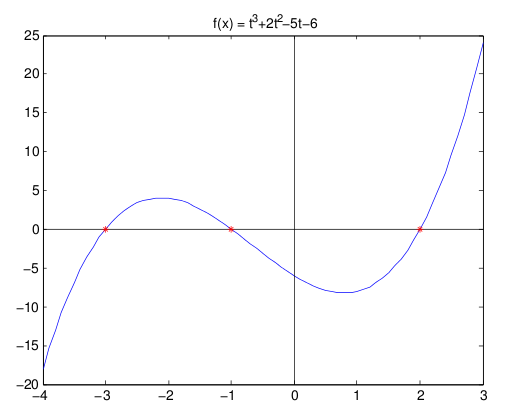
\includegraphics[width=6cm]{img/polinomio.png}
          \label{fig:polinomio}
          \caption{$p(x) = t^3+2t^2-5t-6$ e suas raizes.}
          \end{center}
       \end{figure}
\end{frame}
%%%%%%%%%%%%%%%%%%%%%%%%%%%%%%%%%%%%%%%%%%%%%%%%%%%%%%%%%%%%%%%%%%%%%%%%%%%%%%%%%%%%%%%%%
\begin{frame}
   \frametitle{Sistema de equações não lineares: \code{fsolve}}
 
   Para encontrarmos a solução de um sistema de equações não lineares da forma
   $$F(x) = 0$$
   onde $F:{\mathbb{R}}^n \rightarrow {\mathbb{R}}^m$, usamos a função \acode{fsolve}, identicamente à função \acode{fzero}:
   \codigo{\ac & \acode{fsolve}(@minhafuncao,x0)}
   se utilizarmos uma função em arquivo, ou
   \codigo{\ac & \acode{fsolve}(fun,x0)}
   se utilizarmos uma função anônima.
 
   \vfill
   \alert{Só na \emph{Optimization Toolbox}!}
\end{frame}
%%%%%%%%%%%%%%%%%%%%%%%%%%%%%%%%%%%%%%%%%%%%%%%%%%%%%%%%%%%%%%%%%%%%%%%%%%%%%%%%%%%%%%%%%
\begin{frame}
  \frametitle{Exemplo}
  Resolver o sistema de equações 
  \begin{equation*}
    \begin{cases}
      y_1 &= 3x_1^2+4x_2^2-16\\
      y_2 &= 2x_1^2-3x_2^2-5
    \end{cases}
  \end{equation*}
  
  \codigo{\ac & fun = @(x) [3*x(1).\^{}2+4*x(2).\^{}2-16;\\
    & \hskip2.5cm 2*x(1).\^{}2-3*x(2).\^{}2-5];\\
    \ac & \acode{fsolve}(fun,[1;1])}
\end{frame}
%%%%%%%%%%%%%%%%%%%%%%%%%%%%%%%%%%%%%%%%%%%%%%%%%%%%%%%%%%%%%%%%%%%%%%%%%%%%%%%%%%%%%%%%% 
\begin{frame}
   \frametitle{Exemplo}
   Encontrar a raiz de 
   \begin{equation*}
      F(x) = \begin{bmatrix}
      x_1^2+x_2x_3\\
      sin(x_1+2x_2-3x_3)
   \end{bmatrix}
   \end{equation*}
   \codigo{\ac & fun = @(x) [x(1).\^{}2+x(2).*x(3);\\
     & \hskip2.5cm \acode{sin}(x(1)+2*x(2)-3*x(3))];\\
     \ac & \acode{fsolve}(fun,[1;1;1])\\
     \ac & \acode{fsolve}(fun,[0;0;0])}
\end{frame}
%%%%%%%%%%%%%%%%%%%%%%%%%%%%%%%%%%%%%%%%%%%%%%%%%%%%%%%%%%%%%%%%%%%%%%%%%%%%%%%%%%%%%%%%% 
\begin{frame}
   \frametitle{Otimização: Minimização de funções}
    Agora, queremos resolver o problema
    \begin{equation*}
     \mbox{ minimizar } f(x).
    \end{equation*}
 
    Para encontrarmos o mínimo de uma função real de várias variáveis, a partir
de um ponto inicial \code{x0}, usamos o comando
    \codigo{\ac & x = \acode{fminsearch}(@funcao,x0)}
    Se quisermos também saber o valor da função no ponto de mínimo, usamos a
sintaxe
    \codigo{\ac & [x,fval] = \acode{fminsearch}(@funcao,x0)}
\end{frame}
%%%%%%%%%%%%%%%%%%%%%%%%%%%%%%%%%%%%%%%%%%%%%%%%%%%%%%%%%%%%%%%%%%%%%%%%%%%%%%%%%%%%%%%%%
\begin{frame}
   \frametitle{Exemplo}
   Minimizar
   \begin{equation*}
     f(x) = 100(x_2-x_1^2)^2+(1-x_1)^2
   \end{equation*}
   \codigo{\ac & f = @(x) 100*(x(2)-x(1).\^{}2).\^{}2+(1-x(1)).\^{}2\\
     \ac & \acode{fminsearch}(f,[0;0])}
\end{frame}
%%%%%%%%%%%%%%%%%%%%%%%%%%%%%%%%%%%%%%%%%%%%%%%%%%%%%%%%%%%%%%%%%%%%%%%%%%%%%%%%%%%%%%%%%
% \begin{frame}
%    \frametitle{Exemplo}
%    Minimizar a função 
%    $$f = e^{x_1}(4x_1^2 + 2x_2^2 + 4x_1x_2 + 2x_2 + 1)$$
%    a partir do ponto inicial $x_0 = (0,0)$.
%    \only<2>{\codigo{\ac &
% f=@(x)exp(x(1))*(4*x(1)\^{}2+2*x(2)\^{}2+4*x(1)*x(2)+2*x(2)+1);\\
%    \ac & fminsearch(f,[0;0])}}
% \end{frame}
%%%%%%%%%%%%%%%%%%%%%%%%%%%%%%%%%%%%%%%%%%%%%%%%%%%%%%%%%%%%%%%%%%%%%%%%%%%%%%%%%%%%%%%%%
\begin{frame}
   \frametitle{Minimização de uma função de uma variável com restrições:
\code{fminbnd}}
 
    Para encontrarmos o mínimo de uma função de uma variável dentro de um
intervalo $[a,b]$, usamos o comando
    \codigo{\ac & x = \acode{fminbnd}(@funcao,a,b)}
    Se quisermos também saber o valor da função no ponto de mínimo, usamos a
sintaxe
    \codigo{\ac & [x,fval] = \acode{fminbnd}(@funcao,a,b)}
\end{frame}
%%%%%%%%%%%%%%%%%%%%%%%%%%%%%%%%%%%%%%%%%%%%%%%%%%%%%%%%%%%%%%%%%%%%%%%%%%%%%%%%%%%%%%%%%
\begin{frame}
  \frametitle{Exemplos}
  \begin{itemize}
  \item Minimizar $f(x) = x$ nos intervalos $[0,1]$ e $[-10,1]$.
    \codigo{\ac & f = @(x) x;\\
      \ac & \acode{fminbnd}(f,0,1)\\
      \ac & \acode{fminbnd}(f,-10,1)}
  \item Minimizar $f(x) = x^2-1$ no intervalo $[1,3]$.
    \codigo{\ac & f = @(x) x.\^{}2;\\
      \ac & \acode{fminbnd}(f,1,3)}
  \end{itemize}
\end{frame}
%%%%%%%%%%%%%%%%%%%%%%%%%%%%%%%%%%%%%%%%%%%%%%%%%%%%%%%%%%%%%%%%%%%%%%%%%%%%%%%%%%%%%%%%% 
\begin{frame}
  \frametitle{}
  \begin{center}
    \alert{Outros comandos úteis}
  \end{center}
\end{frame}
%%%%%%%%%%%%%%%%%%%%%%%%%%%%%%%%%%%%%%%%%%%%%%%%%%%%%%%%%%%%%%%%%%%%%%%%%%%%%%%%%%%%%%%%% 
\begin{frame}
   \frametitle{Integração numérica geral: \code{integral}}

   Para calcularmos uma aproximação numérica de $\int_a^b f(x) dx$, usamos o comando
   \codigo{\ac & q = \acode{integral}(fun,a,b)}
   em que \code{fun} é uma referência a uma função.

   \vfill
   Exemplo:

   Calcular a integral imprópria de $f(x) = e^{-x^2}(\ln{(x)})^2$ entre $0$ e $\infty$.
   \codigo{\ac & fun = @(x) \acode{exp}(-x.\^{}2).*\acode{log}(x).\^{}2;\\
     \ac & q = \acode{integral}(fun,0,Inf)}
\end{frame}
%%%%%%%%%%%%%%%%%%%%%%%%%%%%%%%%%%%%%%%%%%%%%%%%%%%%%%%%%%%%%%%%%%%%%%%%%%%%%%%%%%%%%%%%%
\begin{frame}
 \frametitle{Integração numérica finita: \code{quad}}
   Para calcularmos uma aproximação numérica de $\int_a^b f(x) dx$ pela quadratura de Simpson (adaptativa), usamos o comando
   \codigo{\ac & q = \acode{quad}(fun,a,b)}
   em que \code{fun} é uma referência a uma função.
\end{frame}
%%%%%%%%%%%%%%%%%%%%%%%%%%%%%%%%%%%%%%%%%%%%%%%%%%%%%%%%%%%%%%%%%%%%%%%%%%%%%%%%%%%%%%%%%
\begin{frame}
   \frametitle{Integração numérica discreta: \code{trapz}}
   Se tudo o que conhecemos sobre a função é seus valores em um conjunto de pontos, podemos aproximar o valor da sua integral $\int_a^b f(x) dx$ usando o comando \acode{trapz}.
% \codigo{\ac & x = 0:pi/100:pi;\\
%    \ac & y = sin(x);\\
%    \ac & z = trapz(x,y)}
   Para calcularmos uma aproximação numérica de $\int_a^b f(x) dx$, primeiramente precisamos representar a função $f$ em um conjunto de pontos:
   \codigo{\ac & x = 0:pi/100:pi;\\
   \ac & y = \acode{sin}(x);}
   Agora, usamos o comando \acode{trapz}:
   \codigo{\ac & z = \acode{trapz}(x,y)}
\end{frame}
%%%%%%%%%%%%%%%%%%%%%%%%%%%%%%%%%%%%%%%%%%%%%%%%%%%%%%%%%%%%%%%%%%%%%%%%%%%%%%%%%%%%%%%%%
\begin{frame}
   \frametitle{Diferenciação Numérica: \code{gradient}}

   O \emph{gradiente} de uma função $f:{\mathbb{R}}^n \to {\mathbb{R}}$ é dado por
   \begin{equation*}
      \nabla f(x) = \left( \frac{\partial f}{\partial x_1}(x), \frac{\partial f}{\partial x_1}(x), \ldots, \frac{\partial F}{\partial x_n}(x)\right).
   \end{equation*}

   Para calcularmos o gradiente de uma função de uma variável, procedemos da seguinte maneira.

   \codigo{\ac & x = a:h:b;\\
      \ac & f = \acode{funcao}(x);\\
      \ac & g = \acode{gradient}(f,h)}
   
   O comando \acode{gradient} calcula numericamente a derivada de $f$ em função da variável $x$ nos pontos escolhidos. 
\end{frame}
%%%%%%%%%%%%%%%%%%%%%%%%%%%%%%%%%%%%%%%%%%%%%%%%%%%%%%%%%%%%%%%%%%%%%%%%%%%%%%%%%%%%%%%%%
\begin{frame}
   \frametitle{Diferenciação Numérica: \code{gradient}}
   Para calcularmos o gradiente de uma função de duas variáveis, o procedimento é equivalente. A diferença é que agora precisamos gerar uma malha de pontos usando o comando \acode{meshgrid}.
   
   \codigo{\ac & x = a:hx:b;\\
      \ac & y = c:hy:d;\\
      \ac & [x,y] = \acode{meshgrid}(x,y);\\
      \ac & f = \acode{funcao}(x,y)\\
      \ac & [gx,gy] = \acode{gradient}(f,hx,hy)}
\end{frame}
%%%%%%%%%%%%%%%%%%%%%%%%%%%%%%%%%%%%%%%%%%%%%%%%%%%%%%%%%%%%%%%%%%%%%%%%%%%%%%%%%%%%%%%%%
\begin{frame}
   \frametitle{Interpolação}
   Suponha que temos um conjunto de dados, e gostaríamos de encontrar uma função polinomial (ou polinomial por partes) que \emph{interpole} estes pontos.
   \begin{center}
     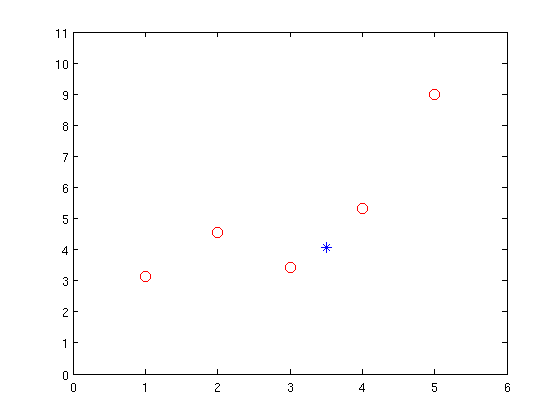
\includegraphics[width=6cm]{img/interpolation.png}
   \end{center}
\end{frame}
%%%%%%%%%%%%%%%%%%%%%%%%%%%%%%%%%%%%%%%%%%%%%%%%%%%%%%%%%%%%%%%%%%%%%%%%%%%%%%%%%%%%%%%%%
\begin{frame}
   \frametitle{Interpolação 1D: \code{interp1}}
   O comando
   \codigo{\ac & yi = \acode{interp1}(x,Y,xi,method)}
   interpola os dados (\code{x},\code{Y}) nos novos pontos \code{xi},
   usando o método \code{method}, que pode ser:
   \begin{itemize}
      \item \code{'nearest'} Vizinho mais próximo
      \item \code{'linear'} Interpolação linear (default)
      \item \code{'spline'} Splines cúbicos
      \item \code{'cubic'} Interpolação por polinômios de Hermite
   \end{itemize}
\end{frame}
%%%%%%%%%%%%%%%%%%%%%%%%%%%%%%%%%%%%%%%%%%%%%%%%%%%%%%%%%%%%%%%%%%%%%%%%%%%%%%%%%%%%%%%%%
\begin{frame}
   \frametitle{Exemplo}
   \codigo{\ac & x = 0:10;\\
      \ac & y = \acode{sin}(x); \\
      \ac & xi = 0:.25:10; \\
      \ac & yi = \acode{interp1}(x,y,xi); \\
      \ac & \acode{plot}(x,y,'o',xi,yi);\\
      \ac & hold on;\\
      \ac & zi = \acode{interp1}(x,y,xi,'nearest');\\
      \ac & \acode{plot}(xi,zi,':k');\\
      \ac & wi = \acode{interp1}(x,y,xi,'spline');\\
      \ac & \acode{plot}(xi,wi,'m');\\
      \ac & ui = \acode{interp1}(x,y,xi,'cubic');\\
      \ac & \acode{plot}(xi,ui,'--g')
	}
\end{frame}
%%%%%%%%%%%%%%%%%%%%%%%%%%%%%%%%%%%%%%%%%%%%%%%%%%%%%%%%%%%%%%%%%%%%%%%%%%%%%%%%%%%%%%%%%
\begin{frame}
   \frametitle{Interpolação 2D: \code{interp2}}
   O comando
   \codigo{\ac & ZI = \acode{interp2}(X,Y,Z,XI,YI,method)}
   interpola os dados (\code{X},\code{Y},\code{Z}) nos novos pontos
   (\code{XI},\code{YI}) usando o método \code{method}, que pode ser
   \begin{itemize}
      \item \code{'nearest'} Vizinho mais próximo
      \item \code{'linear'} Interpolação linear (default)
      \item \code{'spline'} Splines cúbicos
      \item \code{'cubic'} Interpolação cúbica, se os dados forem uniformemente espaçados; senão, é o mesmo que \code{spline}.
   \end{itemize}
\end{frame}
%%%%%%%%%%%%%%%%%%%%%%%%%%%%%%%%%%%%%%%%%%%%%%%%%%%%%%%%%%%%%%%%%%%%%%%%%%%%%%%%%%%%%%%%%
% \begin{frame}
%  \frametitle{Exemplo}
% \end{frame}
% %%%%%%%%%%%%%%%%%%%%%%%%%%%%%%%%%%%%%%%%%%%%%%%%%%%%%%%%%%%%%%%%%%%%%%%%%%%%%%%%%%%%%%%%%
\begin{frame}
  \frametitle{Resolução de Equações Diferenciais}
  Uma EDO é uma equação que envolve uma ou mais derivadas de uma variável dependente $y$ com respeito a uma única variável independente $t$ ($y = y(t)$).

  O MATLAB resolve equações diferenciais ordinárias de primeira ordem dos seguintes tipos:
  \begin{itemize}
  \item EDOs explícitas, do tipo $y' = f(t,y)$
  \item EDOs linearmente implícitas, do tipo $M(t,y)y' = f(t,y)$, em que $M(t,y)$ é uma matriz
  \item EDOs implícitas, do tipo $f(t,y,y') = 0$ %(ode15i only)
  \end{itemize}

Para resolvermos equações diferenciais de ordem superior, precisamos escrevê-las como um sistema de equações de primeira ordem (como fazemos no curso de cálculo).
\end{frame}
%%%%%%%%%%%%%%%%%%%%%%%%%%%%%%%%%%%%%%%%%%%%%%%%%%%%%%%%%%%%%%%%%%%%%%%%%%%%%%%%%%%%%%%%%
\begin{frame}
  \frametitle{Problemas de Valor Inicial}
  Geralmente, temos uma família de soluções $y(t)$ que satisfaz a EDO. Para obtermos uma solução única, exigimos que a solução satisfaça alguma condição inicial específica, de forma que $y(t_0) = y_0$ em algum valor inicial $t_0$.
  \begin{align*}
    \begin{cases}
    y' = f(t,y)\\
    y(t_0) = y_0
    \end{cases}
  \end{align*}
\end{frame}
%%%%%%%%%%%%%%%%%%%%%%%%%%%%%%%%%%%%%%%%%%%%%%%%%%%%%%%%%%%%%%%%%%%%%%%%%%%%%%%%%%%%%%%%%
\begin{frame}
  \frametitle{Solvers}
  A sintaxe para resolver uma equação diferencial é
  \codigo{\ac & [t,y] = \emph{solver}(odefun,tspan,y0,options)}
  Os argumentos de entrada são sempre os seguintes:
  \begin{itemize}
  \item \code{odefun}: O \emph{handle} para uma função que avalia o sistema de EDOs em um ponto. Esta função deve estar na forma \code{dydt = odefun(t,y)}, onde \code{t} é um escalar e \code{dydt} e \code{y} são vetores coluna.
  \item \code{tspan}: vetor especificando o intervalo de integração.
  \item \code{y0}: vetor das condições iniciais para o problema.
  \item \code{options}: Struct de parâmetros opcionais.
  \end{itemize}
  
  Os argumentos de saída são
  \begin{itemize}
  \item \code{t}: vetor coluna das variáveis independentes (pontos no intervalo desejado)
  \item \code{y}: vetor ou matriz contendo, em cada linha, a solução calculada no ponto contido na linha correspondente de \code{t}.
  \end{itemize}
\end{frame}
%%%%%%%%%%%%%%%%%%%%%%%%%%%%%%%%%%%%%%%%%%%%%%%%%%%%%%%%%%%%%%%%%%%%%%%%%%%%%%%%%%%%%%%%%
\begin{frame}
  \frametitle{Solvers}
    Os métodos disponíveis estão divididos de acordo com o tipo de problema que resolvem:
\begin{itemize}
\item Problemas Não-Stiff:
  \begin{itemize}
  \item \acode{ode45} (Runge-Kutta, passo simples)
  \item \acode{ode23} (Runge-Kutta, passo simples)
  \item \acode{ode113} (Adams-Bashforth-Moulton, passo múltiplo)
  \end{itemize}
\item Problemas Stiff:
  \begin{itemize}
  \item \acode{ode15s} (numerical differentiation formulas (NDFs), passo múltiplo)
  \item \acode{ode23s} (Rosenbrock, passo único)
  \item \acode{ode23t} (Trapezoide)
  \item \acode{ode23tb} (Runge-Kutta)
  \end{itemize}
\end{itemize}

Para equações implícitas da forma
\begin{equation*}
  f(t,y,y') = 0, 
\end{equation*}
pode-se usar o solver \acode{ode15i}.
\end{frame}
%%%%%%%%%%%%%%%%%%%%%%%%%%%%%%%%%%%%%%%%%%%%%%%%%%%%%%%%%%%%%%%%%%%%%%%%%%%%%%%%%%%%%%%%%
\begin{frame}
  \frametitle{Exemplo}
  Resolver o problema de valor inicial
  \begin{equation*}
    \begin{cases}
      y'(t) = \cos{t}\\
      y(0) = 0
    \end{cases}
  \end{equation*}
  \vfill
  \codigo{\ac & odefun = @(t,y) \acode{cos}(t);\\
    \ac & [T,Y] = \acode{ode45}(odefun,[0 1],0)\\
    \ac & \acode{plot}(T,Y)\\
    \ac & \acode{hold on}\\
    \ac & \acode{plot}(T,\acode{sin}(T),'m')} 
\end{frame}
%%%%%%%%%%%%%%%%%%%%%%%%%%%%%%%%%%%%%%%%%%%%%%%%%%%%%%%%%%%%%%%%%%%%%%%%%%%%%%%%%%%%%%%%%
% Euler Equations (Nonstiff)


% rigidode illustrates the solution of a standard test problem proposed by Krogh for solvers intended for nonstiff problems [8].

% The ODEs are the Euler equations of a rigid body without external forces.



% For your convenience, the entire problem is defined and solved in a single M-file. The differential equations are coded as a subfunction f. Because the example calls the ode45 solver without output arguments, the solver uses the default output function odeplot to plot the solution components. 

% To run this example, click the example name, or type rigidode at the command line.
% function rigidode 
% %RIGIDODE  Euler equations: rigid body without external forces
% tspan = [0 12];
% y0 = [0; 1; 1];

% % Solve the problem using ode45
% ode45(@f,tspan,y0);
% % ------------------------------------------------------------
% function dydt = f(t,y)
% dydt = [ y(2)*y(3) 
%         -y(1)*y(3) 
%         -0.51*y(1)*y(2) ];
%%%%%%%%%%%%%%%%%%%%%%%%%%%%%%%%%%%%%%%%%%%%%%%%%%%%%%%%%%%%%%%%%%%%%%%%%%%%%%%%%%%%%%%%%
% \begin{frame}
%    \frametitle{Grupos}

%    Com frequência, precisamos agrupar variáveis para facilitar o cálculo de estatísticas e para criar visualizações.
%    \vfill
%    Variáveis de agrupamento tem o mesmo comprimento que as variáveis (colunas) em um conjunto de dados. 
%    \vfill
%    Consideramos que as observações (linhas) $i$ e $j$ estão no mesmo grupo se os valores da variável de agrupamento correspondente forem idênticos nestes índices.
% \end{frame}
%%%%%%%%%%%%%%%%%%%%%%%%%%%%%%%%%%%%%%%%%%%%%%%%%%%%%%%%%%%%%%%%%%%%%%%%%%%%%%%%%%%%%%%%%
% \begin{frame}
%    \frametitle{Grupos: Exemplo}
%    \codigo{\ac & \; dados = \acode{rand}(10,4);\\
%       \ac & \; agrupamento = \acode{cell}{(10,1)};\\
%       \ac & \; \acode{for} i = 1:10\\
%       & \; \; \acode{if} i <= 6\\
%       & \; \; \; agrupamento\{i\} = 'litoral';\\
%       & \; \; \acode{else}\\
%       & \; \; \; agrupamento\{i\} = 'interior';\\
%       & \; \; \acode{end}\\
%       & \; \acode{end}}
% \end{frame}
%%%%%%%%%%%%%%%%%%%%%%%%%%%%%%%%%%%%%%%%%%%%%%%%%%%%%%%%%%%%%%%%%%%%%%%%%%%%%%%%%%%%%%%%%
% \begin{frame}
%   \frametitle{\code{gscatter}}

%   O comando
%   \codigo{\ac & \; \acode{gscatter}(x,y,grupo)}
%   faz um scatter plot diferenciando entre os grupos de dados.
%   \vfill
%   Exemplo:
%   \codigo{\ac & \; \acode{gscatter}(dados(:,1),dados(:,2),agrupamento)}
% \end{frame}
%%%%%%%%%%%%%%%%%%%%%%%%%%%%%%%%%%%%%%%%%%%%%%%%%%%%%%%%%%%%%%%%%%%%%%%%%%%%%%%%%%%%%%%%%
% \begin{frame}
%    \frametitle{\code{gplotmatrix}}

%    O comando
%    \codigo{\ac & \; \acode{gplotmatrix}(x,y,grupo)}
%    cria uma matriz de scatter plots. Cada gráfico dentro da figura contém um scatter plot de uma coluna de \code{x} contra uma coluna de \code{y}. Os gráficos ficam agrupados segundo a variável \code{grupo}.
%    \vfill
%    \code{x} e \code{y} são matrizes com o mesmo número de linhas. 

%    \vfill
%    Exemplo:
%    \codigo{\ac & \; \acode{gplotmatrix}(dados(:,1:2),dados(:,3:4),agrupamento)}
% \end{frame}
%%%%%%%%%%%%%%%%%%%%%%%%%%%%%%%%%%%%%%%%%%%%%%%%%%%%%%%%%%%%%%%%%%%%%%%%%%%%%%%%%%%%%%%%%
% \begin{frame}
%    \frametitle{\code{gplotmatrix}: exemplo}
%    \codigo{\ac & \hspace{-10pt} \acode{load} discrim\\
%       \ac & \hspace{-10pt} \acode{gplotmatrix}(ratings(:,1:2),ratings(:,[4 7]),group)\\
%       \ac & \hspace{-10pt} \acode{gplotmatrix}(ratings(:,1:2),ratings(:,[4 7]),group,... \\
%       & \;\;\; 'br','.o',[],'on','',categories(1:2,:),... \\
%       & \;\;\; categories([4 7],:))}
% \end{frame}
%%%%%%%%%%%%%%%%%%%%%%%%%%%%%%%%%%%%%%%%%%%%%%%%%%%%%%%%%%%%%%%%%%%%%%%%%%%%%%%%%%%%%%%%%
% \begin{frame}
%   \frametitle{Como ignorar NaN automaticamente}

%   Vários comandos da toolbox de Estatística do MATLAB possuem facilidades para se lidar com dados NaN:

%   \begin{itemize}
%      \item \acode{nancov}: Covariância 
%      \item \acode{nanmax}: Máximo
%      \item \acode{nanmean}: Média 
%      \item \acode{nanmedian}: Mediana
%      \item \acode{nanmin}: Mínimo
%      \item \acode{nanstd}: Desvio padrão
%      \item \acode{nansum}: Soma 
%      \item \acode{nanvar}: Variância
%   \end{itemize}
% \end{frame}
\end{document}
